\documentclass{article}
\usepackage{xeCJK}
\usepackage[utf8]{inputenc}
\usepackage{graphicx}
\usepackage{soul}
\usepackage{caption}
\usepackage[utf8]{inputenc}
\usepackage{amsmath}
\usepackage[dvipsnames]{xcolor}
\DeclareMathOperator*{\argmax}{arg\,max}
\DeclareMathOperator*{\argmin}{arg\,min}

\title{Forecasting, decoding and state prediction}
\author{Yun-Hsiang Chan}
\date{June 2021}

\begin{document}

\maketitle
Main results of this chapter: \\
\\
\textbf{Conditional distributions}
$$Pr(X_t = x | X^{(-t)} = x^{(-t)}) = \sum_{i} w_i(t) p_i(x)$$
\\
\textbf{forecast distribution}
$$Pr(X_{T+h} = x | X^{(T)} - x^{(T)}) - \sum_{i} \xi_i(h) p_i(x)$$
\\
\textbf{state probabilities and local decoding}
$$Pr(C_t = i | X^{(T)} = x^{(T)}) = \alpha_t(i) \beta_t(i) / L_T$$
\\
\textbf{global decoding} maximize over $c^{(T)}$ 
$$Pr(C^{(T)} = c^{(T)} | X^{(T)} = x^{(T)})$$
\\
\textbf{state prediction}
$$Pr(C_{T+h} = i | X^{(T)} = x^{(T)}) = \alpha_T \Gamma^h e_i' / L_T$$

\section*{I. Introduction}

In this chapter, we first show how to compute the conditional distribution of the observation at given time t given the observations at all other times. Then we derive the forecast distribution of an HMM. After that, we demonstrate how, given HMM and ther observations, one can deduce information about the stats occupied by the underlying Markov chain. \\
\\
Note that this chapter do not assume stationarity of the Markov chain $\{C_t\}$, only homogeneity. 

\section*{II. Conditional distributions}
We use the notation $X^{(-t)}$ for the distribution of $X_t$ conditioned on all the other observations of the HMM. $x^{(-t)}$ for the observations at all times other than $t$. \\
\\
Using the likelihood of an HMM, 
$$Pr(X_t = x | X^{(-t)} = x^{(-t)}) \propto \alpha_{t-1} \Gamma P(x) \beta_t'$$
\\
Here, we used the compact notation $B_t = \Gamma P(x_t)$. With the notation, $\alpha_t = \delta P(x_1) B_2 ... B_t$ and $\beta_t' = B_{t+1}... B_T 1'$. \\
\\
The conditional distribution are ratios of two likelihoods of HMM \\
1. the numerator is the likelihood of the observations except the observation $x_t$ is replaced by $x$. \\
2. the denominator is the likelihood of the obesrvations except that $x_t$ is treated as missing. \\
\\
We now show that these conditional probabilities can be expressed as mixtures of the m state-dependent probability distributions, i.e.
$$Pr(X_t = x | X^{(-t)} = x^{(-t)}) \propto \sum_{i=1}^m d_i(t) p_i(x)$$ 
where, $d_i(t)$ is the product of the ith entry of vector $\alpha_{t-1} \Gamma$ and the ith entry of the vector $\beta_t$. Hence, 
$$Pr(X_t = x | X^{(-t) = x^{(-t)}} = \sum_{i=1}^m w_i(t) p_i(x))$$
where the mixing probabilties $w_i(t) = d_i(t) / \sum_{j=1}^m d_j(t)$ are functions of the observations $x^{(t)}$ and of the model parameters. 

\section*{III. Forecast distributions}
Forecast distribution is another type of conditional distribution of an HMM. Sepcifically, we derive two expressions for the conditional distribution of $X_{T+h}$ given $X^{(T)} = x^{(T)}$, where $h$ is the forecast horizon. \\
\\
For discrete-valued observations the forecast distribution $Pr(X_{T+h} = x | X^{(T)} = x^{(T)})$ of an HMM is very similar to the conditional distribution $Pr(X_t = x | X^{(-t)} = x^{(-t)})$, and can be computed in the same way:
\\
\begin{align}
    Pr(X_{T+h} = x | X^{(T)} = x^{(T)}) & = \frac{Pr(X^{(T)} = x^{(T)}, X_{T+h} = x)}{Pr(X^{(T)} = x^{(T)})} \\
    & = \frac{\alpha_T \Gamma^h P(x) 1'}{\alpha_T 1'}
\end{align}
Writing $\phi_T = \alpha_T / \alpha_T 1'$, we have 
$$Pr(X_{T+h} = x | X^{(T)} = x^{(T)}) = \phi_T \Gamma^h P(x) 1'$$
\\
The forecast distribution can therefore be written as a mixture of state-dependent probability distributions: 
$$Pr(X_{T+h} = x | X^{(T)} = x^{(T)}) = \sum_{i=1}^m \xi_i (h) p_i(x)$$
where the weights of $\xi_i(h)$ is the ith entry of the vector $\phi_T \Gamma^h$.
\\
Since the entire distribution is known, it is possible to make interval forecasts. As the forsecast horizon h increases, the forecast distributions converges to the marginal distribution of the stationary HMM, 
$$lim_{h \rightarrow \infty} Pr(X_{T+h} = x | X^{(T)} = x^{(T)}) = lim_{h \rightarrow \infty} \phi_T \Gamma^h P(x) 1' = \delta^* P(x) 1'$$

\section*{IV. Decoding}
In speech recognition and other applications, it is of interest to determine the states of the Markov chain that are most likely to have given rise to the observation sequence. \\
\\
\textbf{Local decoding} of the state at time $t$ refers to the determination of that state which is most likely at that time. In constract, \textbf{global decoding} refers to the determination of the most likely sequene of states. 

\subsection*{4.1 State probabilities and local decoding}
Consider again the vectors of forward and backward probabilities, $\alpha_t$ and $\beta_t$. For the derivation of the most likely state of the Markov chain at time $t \in \{1, ..., T\}$, we shall use the following result, which appears there as equation
$$\alpha_t(i) \beta_t(i) = Pr(X^{(T)} = x^{(T)}, C_t = i)$$
Hence, the conditional distribution of $C_t$ given the observations can be obtained, for $i = 1, ..., m$, as \\
\begin{align}
    Pr(C_t = i | X^{(T)} = x^{(T)}) & = \frac{Pr(C_t = i, X^{(T)} = x^{(T)})}{Pr(X^{(T)} = x^{(T)})} \\
    & = \frac{\alpha_t(i)\beta_t(i)}{L_T}
\end{align}
Here, $L_T$ can be computed by the scaling method desribed in Section 3.2. Scaling is also necessary in order to prevent numerical underflow in the evaluation of the product of forward and backward probabilities. \\
\\
Therefore, we can determine the distribution of the state $C_t$ at each time $t$, given the observations $x^{(T)}$. \\
\\
The most porbable state $i_t^*$, given the observations, is defined as
$$i_t^* = \argmax_{i=1, ..., m} Pr(C_t = i | X^{(T)} = x^{(T)})$$
This approach determines the most likely state for each t by maximizing the conditional probability, and is therefore called \textbf{local decoding}.

\subsection*{4.2 Global decoding}

In many applications, such as speech recognition, one is interested not so much in the most likely state for each separate time $t$ as in the most likely sequence of hidden states. \\
\\
Instead of maximizing $Pr(C_t = i | X^{(T)} = x^{(T)})$ over $i$ for each $t$, one seeks that sequence of state $c_1, ..., c_T$ which maximizes the conditional probability 
$$Pr(C^{(T)} = c^{(T)} | X^{(T)} = x^{(T)})$$
or equivalently, and more conveniently, the joint probability
$$Pr(C^{(T)}, X^{(T)}) = \delta_{c_1} \Pi_{t=2}^T \gamma_{c_{t-1}, c_t} \Pi_{t=1}^T p_{c_t} (x_t)$$
\\
This is a subtly different maximization problem from local decoding, and is called global decoding. The results of them are often similar but not identical. \\
\\
Maximizing over all possible state sequences $c_1, ..., c_T$ by brute force would involve $m^T$ function evaluations, which is not feasible for large $T$. Instead, we can use an efficient \textbf{dynamic programming} algorithm to determine the most likely sequence of states, namely Viterbi algorithm. \\
\\
Algorithm: \\
We begin by defining
$$\xi_{1i} = Pr(C_1 = i, X_1 = x_1) = \delta_i p_i(x_1)$$
and for $t = 2, ..., T$
$$\xi_{ti} = \max_{c_1, ...c_{t-1}} Pr(C^{(t-1)} = c^{(t-1)}, C_t = i, X^{(t)} = x^{(t)})$$
\\
It can then be shown that 
$$\xi_{tj} = (\max_{i} (\xi_{t-1}, \gamma_{ij}) p_j(x_t))$$
\\
The required maximizing sequence of state $i_1, ..., i_T$ can then be determined recursively from 
$$i_T = \argmax_{i=1, ..., m} \xi_{Ti}$$
and for $t = T-1, T-2, ..., 1$ from 
$$i_t = \argmax_{i=1, ..., m} (\xi_{ti} \gamma_{i, i_{t+1}})$$
\\
Note that, since the value in global decoding is a product of probabilities, one can choose to maximize its logarithm, in order to prevent numerical underflow.  \\
\\
The codes are in Figure 1.
\begin{figure}
    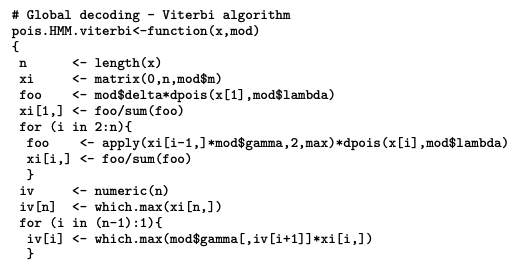
\includegraphics[width = 12cm]{viterbi.png}
    \caption{Viterbi Algorithm}
\end{figure}

\section*{V. State prediction}

Given the observations $x_1, ..., x_T$, the following set of statements can be made about future, present and past states. 

$$L_T Pr(C_t = i | X^{(T)} = x^{(T)}) = \[ \begin{cases} \alpha_T \Gamma^{t - T} e_t' & \text{for $t > T$} \\ \alpha_T(i) & \text{for $t = T$} \\ \alpha_t(i) \beta_t(i) & \text{for $1 \leq t \leq T$} \end{cases}\]$$
where $e_i = (0, ..., 0, 1, 0, ..., 0)$ has a one in the ith position only. 

\section*{VI. HMMs for classification}
This book focuses on the use of HMMs as general-purpose models for time series, that is, the models that encapsulate the main features of the observed series and enable one to extract meaningful information and to forecast. The unobserved states in the model are regarded as artefacts that are uesful but nee not have substantive interpretations\\
\\
In contrast, primarily in the engineering literature, HMMs are often applied solely for the purpose of classifying observations on the state-dependent process into real states. \\
\\
The classic example is in speech recognition, where the states are phonemes that need to be decoded from recorded speech. \\
\\
In such applications one usually begins by taking a training sample in which both the states and the state-dependent observations are recorded. One then estimates the parameters of the model by maximizing the complete-data log-likelihood. The fitted model is used to determine the states that are most likely for new series whose states are unobserved. That step involves decoding states for the series given the trained HMM. \\
\\
In contrast, in the methods and applications covered in this book, the role of states is almost always completely data-driven. 

\end{document}